\documentclass[10pt,twocolumn,letterpaper]{article}

\usepackage{ijcb}
\usepackage{times}
\usepackage{epsfig}
\usepackage{graphicx}
\usepackage{amsmath}
\usepackage{amssymb}
\usepackage{mathtools}
\usepackage{cite}
\usepackage{algpseudocode}

\usepackage{url}
\urldef{\mailsa}\path|thomas.bergmueller@authenticvision.com| 
\urldef{\mailsb}\path|uhl@cosy.sbg.ac.at|
\newcommand{\keywords}[1]{\par\addvspace\baselineskip
\noindent\keywordname\enspace\ignorespaces#1}



\providecommand{\myceil}[1]{\left \lceil #1 \right \rceil }
\providecommand{\myfloor}[1]{\left \lfloor #1 \right \rfloor }







% Include other packages here, before hyperref.

% If you comment hyperref and then uncomment it, you should delete
% egpaper.aux before re-running latex.  (Or just hit 'q' on the first latex
% run, let it finish, and you should be clear).
%\usepackage[pagebackref=true,breaklinks=true,letterpaper=true,colorlinks,bookmarks=false]{hyperref}

%\ijcbfinalcopy % *** Uncomment this line for the final submission

\def\ijcbPaperID{****} % *** Enter the IJCB Paper ID here
\def\httilde{\mbox{\tt\raisebox{-.5ex}{\symbol{126}}}}

% Pages are numbered in submission mode, and unnumbered in camera-ready
\ifijcbfinal\pagestyle{empty}\fi
\begin{document}

%%%%%%%%% TITLE
\title{Impact of sensor aging on iris recognition}

\author{First Author\\
Institution1\\
Institution1 address\\
{\tt\small firstauthor@i1.org}
% For a paper whose authors are all at the same institution,
% omit the following lines up until the closing ``}''.
% Additional authors and addresses can be added with ``\and'',
% just like the second author.
% To save space, use either the email address or home page, not both
\and
Second Author\\
Institution2\\
First line of institution2 address\\
{\tt\small secondauthor@i2.org}
}

\maketitle
\thispagestyle{empty}

%%%%%%%%% ABSTRACT
\begin{abstract}
   Similar to the impact of aging on human beings, digital image sensors develop aging effects over time. Since these imager's aging effects (commonly denoted as pixel defects) leave marks in the captured images, it is not clear whether this affects the accuracy of iris recognition algorithms. This paper proposes a method to investigate the influence of sensor aging on iris recognition by simulative aging of an iris test database. A pixel model is introduced and an aging algorithm is discussed to create the test database. To establish practical relevance, the simulation parameters are estimated from the observed aging effects of a real iris scanner over the timespan of 4 years.
\end{abstract}

%%%%%%%%% BODY TEXT



\section{Introduction}
% TODO probably start with a quote
The aging process starts immediately after being given birth. At first, aging's aspects are considered to be rather positive. One grows up, gets stronger and learns new things. At a certain point, aging starts to reveal several drawbacks. The skin gets wrinkled, joints and bones start to ache and also our vision starts to degenerate. In either case, aging changes parts of our body. Although human beings change, others are still able to recognize people they knew before, even when they haven't met in a long time and therefore aging changed their appearance significantly.
Biometric systems aim to identify human beings by analysing their biometric samples, i.e. the face, the fingerprints or iris \cite{rathgeb}. These systems operate in two steps. In the enrollment process, a subject's biometric samples are registered for the first time and stored in a database. Later, in the authentication procedure, another sample of a subject's biometric samples is taken and compared to the one stored in the database to verify the subject's identity. \\
Since there may be years or decades between the enrollment and the authentication, one strives to use biometric samples which are stable over time. The iris has widely been assumed to be stable, although it is currently topic of intensive discussion if and which iris-related information eventually changes in a human's aging process. Some researchers claim that iris-related information is stable or relatively stable \cite{daugmanPatent, daugmanNoChange, grotherStability, monroDCTIris}, while others observe significant changes over time \cite{rankinChange, rankinChangeResponse, fenkerIrisAging, czajkaTemplateAging, fairhurstNonstability}. Researchers mostly conclude these age-dependent changes in iris texture by observing changes in a system's iris-recognition rate. It is not clear, if observed changes in an algorithms' behaviour are caused by the aging of the tested subject, which is commonly assumed, aging of the recognition system itself or if this is caused by other unspecified factors.

This paper proposes a method to investitage the influence of aging effects of digital image sensors, which are crucial components of the recognition system. As a human being's vision often gets weaker with age, pixels start to get defective in image sensors over the years as well. This influences the quality - and therefore the appearance - of the captured images. Similar to being able to estimate a human being's age by their appearance, pixel defects observed in the captured images can reveal the age of the corresponding imager. This is used in image forensics to approximate the capturing date of an image \cite{fridrich}. However, since the aging effects of the sensor can be traced by evaluation of its output, namely the images, this implies that the capturing process is not time invariant. Hence two images, which capture the same (unchanged) scene, but were taken at significantly different points in time, may differ due to developed sensor defects in the meantime.

% TODO rephrase
There might arise problems due to sensor aging, because iris recognition systems operate by comparing current samples to earlier taken ones stored in a database. Special cameras with digital image sensors are commonly used to capture the iris features in both cases, the enrollment and the authentication process. It is not clear yet, whether the aging of the sensor - and thus the development of aging effects between taking two samples - influence the accuracy of iris recognition algorithms. To investigate this issue, one would need to have identical data captured at at least two significantly different points in time. It is practically impossible to establish identical conditions for both shots. Furthermore, as mentioned, it is not possible to distinguish between the influence of the subject's and the sensor's aging on iris recognition algorithms. For this reason one cannot capture test data to investigate the sensor's or the subject's aging in an isolated manner physically. There is no way to explicitely examine the iris texture's aging at all. However, it is possible to investigate the sensor aging's influence on the iris recognition rate independent from the subject's aging.

%TODO Check Notredame for one sensor only
We proposes a method to investigate the impact sensors aging on the iris recognition rate. This is done by generating simulatively aged test data, which contains sensor aging related defects, based on an uncompressed iris database \cite{iitd} (see section \ref{virtualAging}). The practical relevance of the simulation is ensured by estimating parameters from an iris databases (section \ref{hotPixelRate}), where the same subjects were captured by the same sensor in 2009 and 2013 (section \ref{testing}). This test data set is used to test six implementations of iris recognition algorithms available in the University of Salzburg Iris Toolkit (USIT) \cite{usit}. By observing changes in the EER for certain algorithms, we conclude on the impact of sensor aging on iris recognition systems in section \ref{conclusion}.


\section{Sensor aging and pixel model}
\label{sec:agingAndPixelModel}
An image sensor is a two dimensional array of photosensitive cells called pixels. The purpose of an image sensor is to convert the incoming light to its digital representation, which is commonly denoted as the image \cite{imageSensors}. In theory, each of these pixels has the same rectangular shape and a unified photo-response, meaning all pixels should produce the same output value on unified incoming light. Due to imperfections in the manufacturing process, this is not the case in practice, hence there are pixels which are more sensitive than others \cite{camAndDisplays}. Besides that, some of a sensor's pixels might change their initial photo-response characteristics over the lifetime of a sensor. We denote this defect-development over time as \emph{sensor aging}.
Related work shows that such pixel defects caused by aging are uniformly distributed and independent throughout the sensor. Furthermore, it is well known that the development of pixel defects linked to material-related faults is an increasing function of time \cite{datingImages, inFieldDefects, defectDetection,failureSemi, defectIdentification, fridrich}.

\begin{figure}
\centering
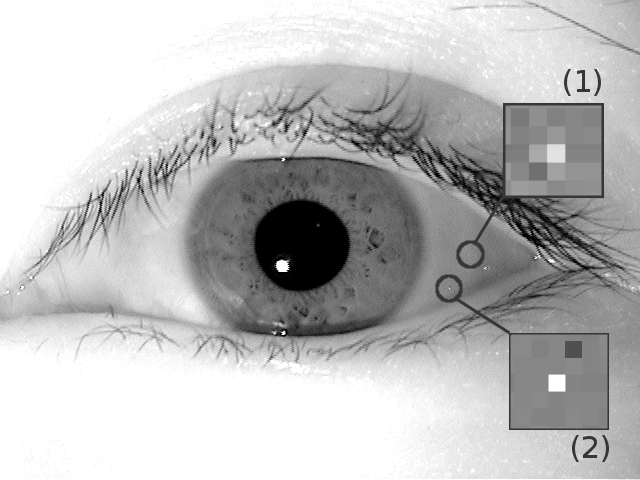
\includegraphics[width=0.7\linewidth]{img/defects.png}
\caption{A \emph{partially-stuck or hot pixel} (1) and two \emph{stuck pixels} (2) in an iris image. Contrast has been enhanced in the close-ups for visualisation. Note that the partially-stuck pixel still corresponds to the incoming light, but is significantly brighter compared to its neighbours, while the stuck pixel are light-independent and yield to a constant output.  }
\label{fig:hotStuck}
\end{figure}

The most common defects occuring over time are partially and fully stuck pixels, illustrated in fig. \ref{fig:hotStuck}. Partially-stuck pixels tend to have a moderate, but still respond to the incident light. Stuck pixels produce a completely light-independent output value and are often (but necessarily) saturated \cite{fridrich}. As soon as a pixel is defective, it remains defective over the rest of the sensor's lifetime \cite{failureSemi}, regardless which type of defect it suffers from. So one can obtain the important property that if a pixel is \emph{once defective, it remains defective}. This is shown in fig. \ref{fig:defectLocations}.

\begin{figure}
\centering
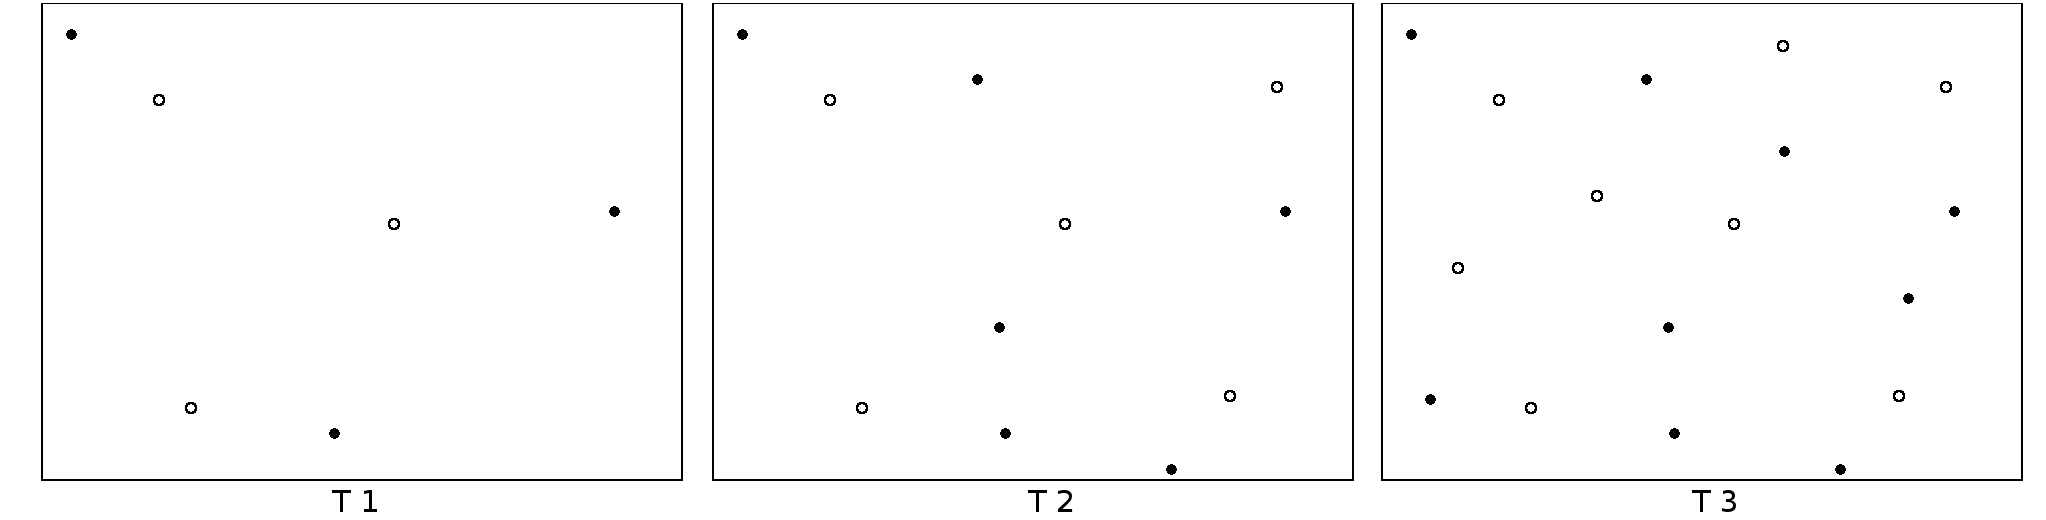
\includegraphics[width=\linewidth]{img/defectLocations.png}
\caption{Illustration of uniformly distributed and independent locations of partially-stuck (circle) and stuck (filled circle) pixels in images taken at 3 significantly different points in time T1, T2, T3.}
\label{fig:defectLocations}
\end{figure}

The occurrence of new pixel defects can be modelled as a poisson process, because the number of pixel defects is increasing linear with time. Defect locations are uniformly distributed and independent. Already known defects remain constant in respect to their location and type \cite{fridrich, defectIdentification}. 
To run a simulation, a model for calculating the pixel values of an image $y$ has to be defined. There are several pixel output models around, which consider the incoming light and the impact of pixel defects on the raw output of a sensor. We denote $w,h \in \mathbb{Z}$ as the rows and columns of the sensor and start by adopting the model proposed in \cite{fridrich}:

\begin{equation}
\begin{aligned}
 Y = I+I \circ K+\tau D +c+\Theta \\ with \quad Y,I,K,D,C, \Theta \in \mathbb{R}^{w \times h}; \tau \in \mathbb{R}
\end{aligned}
  \label{equ:pixelmodel}
 \end{equation}

where $Y$ is the sensor output, commonly denoted as image, $I$ the intensity of incoming light, $I \circ K$ the photo-response non-uniformity PRNU, $\tau D$ the dark current (with $\tau$ being a multiplicative-factor representing exposure settings, sensor temperature, \dots), $C$ a light-independent offset and $\Theta$ some modeling noise. Since all pixels are independent \cite{fridrich, defectDetection} and all operations element-wise, we denote the matrix-elements $y_{x,y} \in Y$ as $ y \in Y$ for simplicity reasons. The same applies to $i \in I$, $k \in K$, $d \in D$, $c \in C$ and $\theta \in \Theta$.\\
Since we're interested in simulating the aging effects of a specific sensor, all age-independent defects, which are e.g. due to production process, can be eliminated. Hence the PRNU, which corresponds to the non-uniformity of pixel-dimensions, can be omitted. As we're interested in reproducable tests, this means environmental influence (e.g. temperature) and modelling noise should be minimized. They can be eliminated completely in a simulation, thus we set $k=\theta=0$. Also the same exposure settings have to be used for the sensor in every test, therefore we have $\tau = const$ and set $ \tau = 1$ for simplicity. \cite{camAndDisplays, radiometricCCD,failureSemi,fridrich} suggest that the dark current is very weak with short exposure, which is necessary for applications in biometric systems to avoid motion blur. Under these considerations, a fairly simple model, considering only aging-relevant defects, remains:

\begin{equation}
  \label{equ:pixemodelEasier}
  y = i + d + c \quad with \quad y,i,c \in \mathbb{R}
\end{equation}

Common defect types that develop over time as the sensor ages are stuck and hot pixels, where the definitions are quite contrary in literature (e.g. in \cite{fridrich, defectIdentification, failureSemi}). If the dark current $d$ of a pixel is extremely high, this is often denoted as a hot pixel. If the offset $c$ is high, this results in a saturated pixel and is called a stuck pixel according to \cite{fridrich}. \cite{defectIdentification}, however, suggests that a stuck pixel is not necessarily saturated but can obtain any value within the sensor output's universe. For the reason of non-uniform definitions we define the following models for defective pixels:

\begin{eqnarray}
  y & = & c \label{equ:Stuck} \\
  y & = & i + d \label{equ:Hot}
\end{eqnarray}
  
where the defect type in equ. \ref{equ:Stuck} is light-independent (thus referred as a \emph{stuck pixel}) and the one in equ. \ref{equ:Hot} adds an offset to the incident light and is commonly referred as either a partially-stuck or hot pixel. The dark current (which is the cause for hot pixels) depends on exposure time and temperature, which are both kept constant this experiment. Thus also the dark current is constant and therefore there is no difference between a hot and a partially stuck pixel for this setup. We will denote this effect as a \emph{partially-stuck pixel}. In conclusion (and considering 8 bit grayscale images), the following pixel model is definied:

\begin{equation}
\begin{aligned}
Y_{x,y} = \begin{cases}
C_{x,y}  & \text{if $c_{x,y} \neq 0$}; \\
I_{x,y} +D_{x,y}  & \text{otherwise}.\\
\end{cases} \\ \text{with} \quad Y,C,I,D \in {(\mathbb{Z}:[0;255])}^{w \times h}
\label{equ:finalPixelModel}
\end{aligned} 
\end{equation}

where $Y_{x,y}$-values are clipped at $0$ and $255$ respectively if interval borders are exceeded. This means they are able to saturate. 

\section{Simulated sensor aging}
\label{virtualAging}
For an ideal sensor, the defect matrices $C$ and $D$ are time-invariant zero matrices. For real sensors, pixel defects start to occur from a specific point in time $T_0$ with a constant rate. This can be modelled by a poisson process \cite{fridrich}. Hence the number of stuck and partially-stuck pixels, denoted as $n_{s}$ and $n_{ps}$ respectively, at $T_i$ can be calculated as

\begin{eqnarray}
   n_s(t)  & = & (T_i-T_0) \lambda_s \\
  n_{ps}(t) & = &  (T_i-T_0) \lambda_{ps}
\end{eqnarray}

where $\lambda_s$ and $\lambda_{ps}$ are the rates at which the particular defect types occur. Due to defects being independent of each other, the locations of the defects among a 2D sensor array can be modelled by a uniform distribution. Thus the defect location $(x,y)$ can be obtained using random numbers $r$. We propose the following procedure to obtain the position $s_k \in {w \times h}$ of the $k$-th pixel defect:

\begin{equation}
 s_k = (\myfloor{\frac{r}{w}}, (r \mod{w})) \quad \text{with} \quad r \in [0:w \cdot h]
 \label{equ:defectLocation}
\end{equation}

Depending on the $k$-th defect being a stuck or partially stuck pixel, the values of $C$ and $D$ (see equ. \ref{equ:finalPixelModel}) have to be set. We denote $a_s$ as the maximum amplitude of a stuck pixel and $a_{ps}$ the maximum amplitude of a partially stuck pixel. Let $r_a \in \mathbb{R}:[0;1]$ be a uniformly distributed random number. Then we either have

\begin{eqnarray}
   C_{s_k}  & = & r_a  a_s \quad \text{for a stuck pixel at } s_k \text{ or} \label{equ:stucks} \\
   D_{s_k} & = &  r_a a_{ps} \quad \text{for a partially-stuck pixel at } s_k \label{equ:partiallyStuck}
\end{eqnarray}

These definitions are used, according to the pixel model in equ. \ref{equ:finalPixelModel}, to add aging-related sensor defects to an existing image $Y_{T_0}$, which was captured at ${T_0}$. One might argue that $Y_{T_0}$ already contains pixel defects since the used sensor might bear defects at $T_0$ already. Since we are only interested in investigating changes over a period of time, it does not matter which time frame we observe. This means, already contained defects in $Y_{T_0}$ do not influence the outcome of the experiment because we get relative results only. Sensor defects corresponding to a sensor's physical condition at a specific time $T_i$ are embedded in the image $Y_{T_0}$. The resulting image $Y_{T_i}$, denoted as \emph{aged image}, captures the same scene as in $T_0$, but bears the impact of aging defects occured over time ${T_i} - {T_0}$. To investigate the behaviour of iris recognition algorithms, we compute a sequence of aged images $(Y_{T_i})_{i=1 \dots m}$. To do so, first a series of defect matrices, which represent the state of aging at a specific point in time $T_i$, is computed. We denote these sequences gfor sample points $T_0$ \dots $T_m$ as

\begin{equation}
\begin{aligned}
(D_{T_i})_{i=0..m} \text{ and } (C_{T_i})_{i=0..m} \\ 
\text{with} \quad C_{T_i}, D_{T_i} \in {(\mathbb{Z}:[0;255])}^{w \times h}
\end{aligned}
\end{equation}

The following algorithm is proposed to compute the sequence of aged images $Y_{T_i}$ for sample points $T_0$ \dots $T_m$ from a source image $Y_{T_0}$:

\vspace{5mm}
\begin{algorithmic}[1]

\Procedure{AgedImageSequence}{$Y_{T_0}$}

\For{$i=1 \dots m$}
\State $\Delta n_s\gets n_s(T_i - T_0) - n_s(T_{i-1} - T_0) $ 
\State $\Delta n_{ps}\gets n_{ps}(T_i - T_0) - n_{ps}(T_{i-1} - T_0) $
\State $D_{T_i}$ = $D_{T_{i-1}}$
\State $C_{T_i}$ = $C_{T_{i-1}}$

  \For{$k=1 \dots \Delta n_s$}
    \State $r_a \gets$ random in $[0;1]$
    \State $s_k \gets$ random in $w \times h$ (equ. \ref{equ:defectLocation})
    \State $C_{T_{i}}(s_k) \gets r_a \cdot a_s$ (equ. \ref{equ:stucks})
  \EndFor
  
  \For{$k=1 \dots \Delta n_{ps}$}
    \State $r_a \gets$ random in $[0;1]$ 
    \State $s_k \gets$ random in $w \times h$ (equ. \ref{equ:defectLocation})
    \State $D_{T_i}({s_k}) \gets r_a \cdot a_{ps}$ (equ. \ref{equ:partiallyStuck})
  \EndFor
  
  
  $Y_{T_{i_{x,y}}} = \begin{cases}
  C_{i_{x,y}}  & \text{if $C_{i_{x,y}} \neq 0$}; \\
  Y_{T_{0_{x,y}}} +D_{i_{x,y}}  & \text{otherwise}.
  \end{cases}$
  
\EndFor
\State \textbf{return} $(Y_{T_i})_{i=1 \dots m}$
\EndProcedure
\end{algorithmic}

\vspace{5mm}


The defect matrices $D$ and $C$ are computed recursively. This is necessary to satisfy the \emph{once defective, always defective} condition. This ensures earlier developed defects are maintained over virtual age. The number of defects, which has to be added to the ones in the previous step, $\Delta n_s$ and $\Delta n_{ps}$ is calculated in each step. Based on this number, location and amplitude for the $i$-th aging step are computed using random numbers. The defect matrices $C_{T_i}$ and $D_{T_i}$ are used to compute an aged image $Y_{T_i}$. Instead of the incident light $I$, the base image $Y_{T_0}$ can be used due to the given arguments of relative evaluation. With this algorithm we obtain a sequence  of aged images $(Y_{T_i})_{i=1 \dots m}$. Each pixel $y_{T_i}$ in this sequence stores the incident light as in $Y_{T_0}$. Additionally it carries information related to the developed age-dependent defects in the time span $T_i-T_0$.
 
 
 
 
 \subsection{Parameter estimation from iris databases}
 \label{hotPixelRate}
 For the discussed simulative aging process, the defect's growth rate and amplitudes have to be defined. In laboratory set-ups hot and \emph{partially stuck pixels} are usually identified by dark calibration tests (i.e. $I=0$) \cite{defectIdentification}. To the best of the authors' knowledge, there is no suitable laboratory-captured data set available for iris imagers. There are databases \cite{czajkaTemplateAging} available, which were acquired using the same equipment at two significantly different dates for the purpose of investigating iris texture aging. In the following we propose a method to retrieve the growth rate and amplitudes of partially-stuck and fully stuck pixels from such databases.

For the pixel model defined in equ. \ref{equ:finalPixelModel}, the growth rate and amplitudes of partially and fully stuck pixels have to be detected. As discussed, this type of defect is usually detected from a single image when the incident light I is simply set to an uniform and known value, i.e. $I=0$. Hence only the defects $\Xi = D+C = Y-I$ remain. Because in our database $I$ is unknown, a statistical approach has to be used.
We denote $Y_0 \dots Y_K$ a sequence of $K$ images taken in a very short period of time. A partially-stuck pixel at position $(x,y)$ adds an light-independent offset to each pixel output $y_k = Y_k({x,y})$ on this position (refer equ. \ref{equ:finalPixelModel}). A \emph{stuck pixel} obtains the same value in each image in this sequence. Hence a pixel at position $(x,y)$ is identified as being stuck iff

\begin{equation}
y_{0} = y_{1} = \dots = y_{K} \label{equ:conditionStuck}
\end{equation}

To find partially stuck pixels, we compute a pixel's mean $\bar{y}$ from the sequence of images:
\begin{eqnarray}
\bar{y} & = & \frac{1}{K}\sum\limits_{k=1}^{K}y_k \\
\bar{y} & = & \frac{1}{K}\sum\limits_{k=1}^{K}(y_k+d+\theta_k) \label{equ:modelWithNoise} \\
\bar{y} & = & d+\frac{1}{K}\sum\limits_{k=1}^{K}(y_k) = d + \mu \label{equ:modelWithD}
\end{eqnarray}
Equ. \ref{equ:modelWithNoise} is obtained by using the pixel model in equ. \ref{equ:finalPixelModel} (without $c$, as shown before, stuck pixels can be ruled out already) and adding some modelling noise $\theta$. Since $d$ denotes a partially-stuck pixeland therefore contained in every one of the sequences images, it is independent of k. The mean of a uniformly distributed modelling noise $\theta$ cancels out for sufficiently large K. We get equ. \ref{equ:modelWithD}, were $\mu$ denotes the mean value over all pixel values $y_k$ in the sequence.

The mean $\bar{y}$ at a certain location has the same value as if taken the median over several $\bar{y}_i$ in its local neighbourhood with distance $q$. This holds if the neighbouring pixels ${y_i}$ in a $q \times q$ neighbourhood had similar pixel values in the original images $Y_i$. Therefore we have the identity $med(y,q) = \bar{y}$, even if one (but less than half) of the $\bar{y}i$ in the neighbourhood is significantly different. Hence sparse pixel defects, which contribute to the mean, disappear when applying median filtering on the mean image's pixels $\bar{y}$ in a local neighbourhood. Considering only parts of the mean image $\bar{Y}$, where mostly unified brightness and texture is present in $Y_1 \dots Y_K$ we derive the partially-stuck pixel estimator $\hat{d}$ from equ. \ref{equ:modelWithD} as

\begin{eqnarray}
\hat{d} = \frac{1}{K}\sum\limits_{k=1}^{K}y_k - med(\bar{y},q \times q) \label{equ:d}
\end{eqnarray}


\begin{figure}
  \centering
  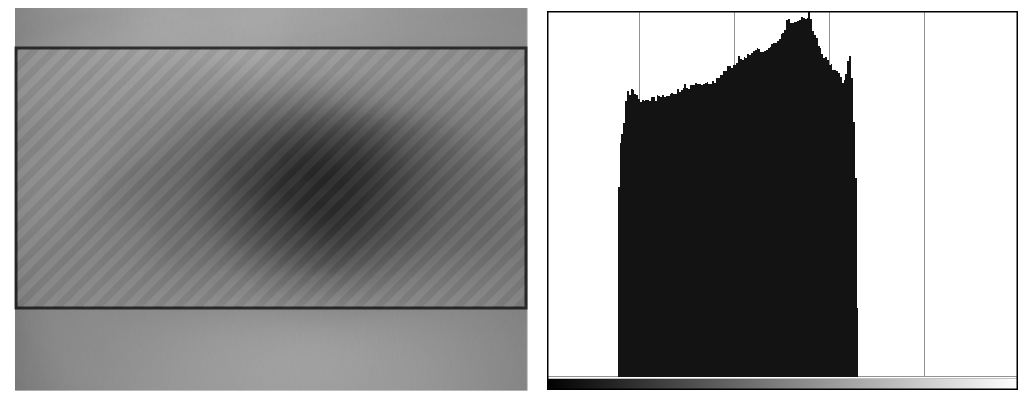
\includegraphics[width=\linewidth]{img/correlated.png}
  \caption{The mean image of $Y_1 \dots Y_k$ (left) has correlated data in the image's centre because of the iris usually being there. This (marked) region is not considered when detecting sensor defects. The histogram (right) of the uncorrelated top and bottom regions is indeed similar to uniform distribution}
  \label{fig:correlated}
\end{figure}

Amongst the partially stuck pixel information, also information about the PNRU is also contained in $\hat{D}$. Since PNRU is caused by imperfections in the manufacturing process, it is likely to be normally distributed which reflects in the logarithmic histogram of $\hat{D}$, as shown in fig. \ref{fig:defectMat}. The size $q$ has to be chosen large enough to minimize the influence of PNRU on the median $med(\bar{y},q)$, which is the case if a normal distribution within the neighbourhood is observed.

\begin{figure}[h]
  \centering
  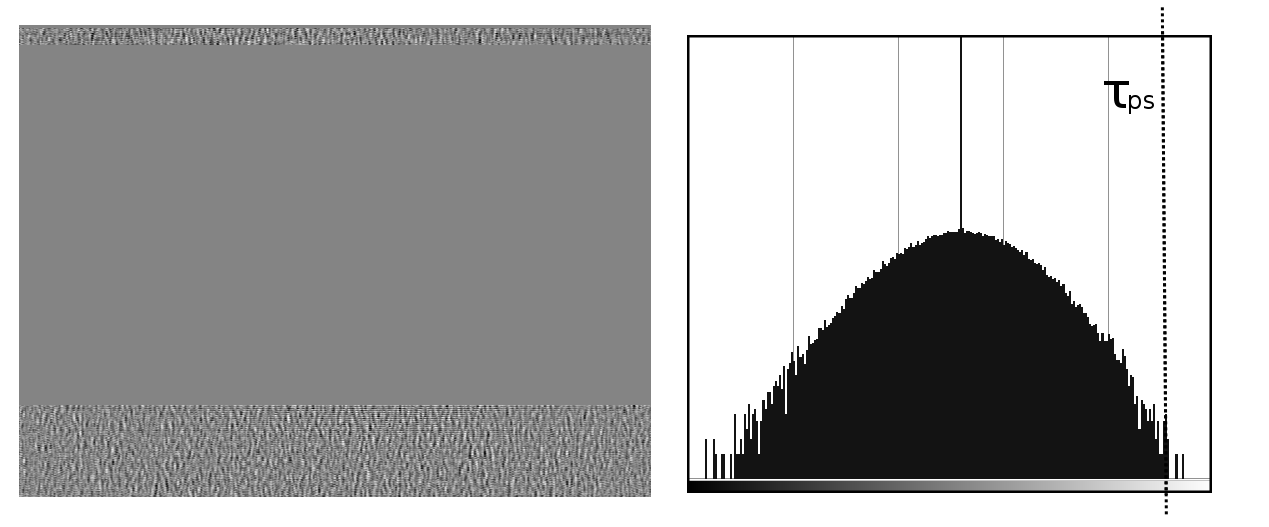
\includegraphics[width=\linewidth]{img/defectMatWithTau.png}
  \caption{Matrix D (left, enhanced for visualisation) is calculated by equ. \ref{equ:d}. The logarithmic histogram (right) of the uncorrelated regions shows a normal distribution, which is due to PNRU. The decision threshold $\tau_{ps}$ is so that only outliers are declared as partially stuck pixels}
  \label{fig:defectMat}
\end{figure}


We declare a pixel to be partially stuck if $\hat{d}$ is an outlier and therefore higher sensivitiy is unlikely to correspond to PNRU. This is decied by checking for a certain threshold $\hat{d} > \tau_{ps}$. The decision threshold is chosen, i.e. manually, to just get approximately same amount of outliers in $T_1$ and $T_2$. We exploit the \emph{once defective, always defective}-property to guarantee correct results, even if $\tau_{ps}$ has been slightly off. We know that a sensor's partially stuck pixels from $T_1$ also have to be present in $T_2$. This is illustrated in fig. \ref{fig:defectPersistence}. The number of defects $n_{match}$, which are present at the same location $s_k$ in the images captured at $T_1$ and $T_2$ can be determined. Considering the number of defects $n_1$ in the image captured at $T_1$, the correction factor $\gamma$ of the algorithm can be calculated as
\begin{equation}
\gamma = \frac{n_{match}}{n_1}
\end{equation}

Assuming that for $T_1$ and $T_2$ the same error is made, the observed increase of defects can be corrected with $\gamma$. Taking into account the size of the sensor $w\cdot h$, we retrieve the simulation parameters by the following relations: 

\begin{figure}
  \centering
  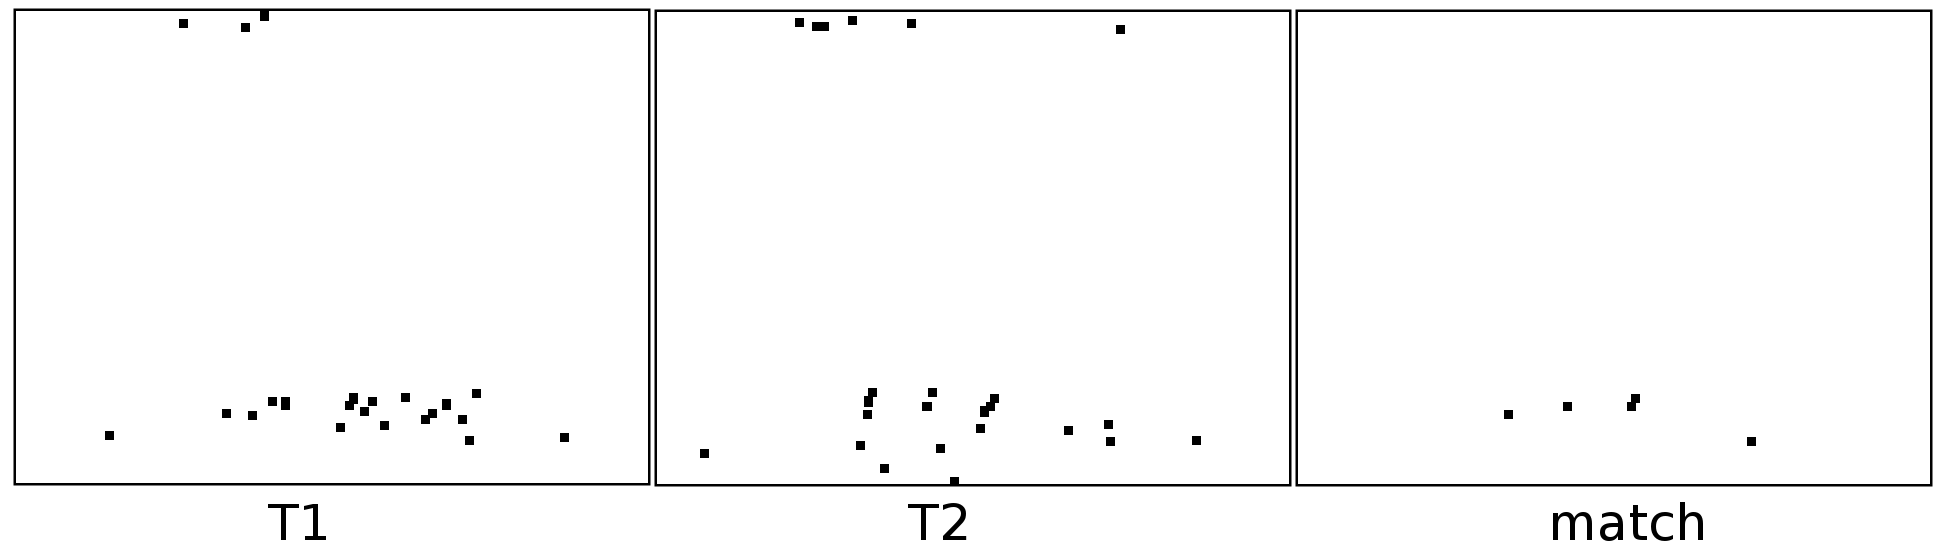
\includegraphics[width=\linewidth]{img/detectedLocations.png}
  \caption{Locations of partially-stuck pixel candidates. Correctly classified pixel defects from $T_1$ are contained in $T_2$ as well. All other detected defects in $T_1$ can be interpreted as misclassification, since they violate the \emph{once defective, always defective}-condition.}
  \label{fig:defectPersistence}
\end{figure}


\begin{eqnarray}
 \lambda_{ps} 	& = 	& \gamma \frac{n_2-n_1}{(T_2-T_1)\cdot(w \cdot h)} \\ 
 \lambda_{s} 	& = 	& \gamma  \frac{n_{s2}-n_{s1}}{(T_2-T_1)\cdot(w \cdot h)} \\
 a_{ps} 	& = 	&max(\hat{D}_{s_k}) \\ 
 a_{s} 		&:= 	& 255
\end{eqnarray}

% TODO: Debiasi14a fehlt...

%%%%%%%%%%%%%%%%%%%%%%%%%%%%%%%%%%%%%%%%%%%%%%%%%%%%%%%%%%%%%%%%%%%%%%%%%%%%%%%%%%%%%%%%%%%%%%%%%%%%%%%%%%%
\section{Experimental setup}
 \label{testing}
 With proposed method simulation parameters are estimated from a dataset. The dataset used in this work contains iris texture images of acquired with the \emph{Irisguard H100 IRT} sensor. The images are divided into 2 data sets, the first one containing images from 49 distinct subjects acquired in 2009, the second one containing images from the exactly the same subjects acquired in 2013, resulting in a time gap of four years between the acquisition of the two image sets. These data sets are subsequently denoted as \emph{H100-2009} and \emph{H100-2013}. \emph{H100-2009} is a subsets of the publicly available CASIA V.3 database.

To be able to reliably estimate the sensor defect's growth rate and amplitudes for the mentioned data sets it is essential to ensure that the image sets in 2009 and 2013 have been acquired using an identical iris sensor device (this is of particular interest since doubts on this issue emerged in the context of the CASIA V.4 datasets recently \cite{Debiasi14a}). 
%Therefore we needed to verify that the \emph{Irispass-2009} and \emph{Irispass-2013} data sets have been acquired with the exactly same iris sensor device, as well as the \emph{H100-2009} and \emph{H100-2013} data sets. 
For this purpose we employ digital image forensic \cite{farid-spm-09} techniques. Sensor fingerprints, a methodology classically used in digital image forensics, are based on a sensor’s photo response non uniformity (PRNU) \cite{12696519,journals/tifs/ChenFGL08} and can be used to prove sample data authenticity by identifying the source sensor uniquely. Even various sensors from the same make/brand and model can be distinguished.

To prove that the sensor device used in 2013 is the same specific device as used in 2009 and vice versa, we adopted the sensor identification methodology of H\"oller and Uhl \cite{UhlH12}. 
We assume that the images under investigation, namely the 2009 and 2013 data sets, are acquired with different sensor devices and derive from the results that this assumption is not correct (proof by contradiction).

We extract the PRNU noise residual of every image from 4 patches located in the corners of the image with a size of 128x128 pixels each. Then from each data set, 2009 and 2013, 850 images are randomly chosen, resulting in a total of 1700 images. From the 850 images per set 50 are used to generate the PRNU fingerprint $\hat{K}$ for the data sets and the other 800 are used to calculate the normalized cross correlation (NCC) scores between fingerprints and noise residuals. 
% At this, the presence of the PRNU fingerprint $\hat{K}$  in the images is examined to obtain the NCC scores.
This leads to 800 matching (fingerprint $\hat{K}$ comes from the same sensor as the images in the data set under investigation) and 800 non-matching NCC scores (fingerprint $\hat{K}$ comes from an other sensor as the images in the data set under investigation) for each sensor.
We then calculate the equal error rate EER from all correlation values $\rho$ by comparing the two data sets. To estimate the real variability of these values, the interval of confidence (CI) at 95\% is estimated. To do so, the calculation of EER and threshold is repeated 1000 times on the respective set of $m$ matching and $n$ non-matching $\rho$ values, by drawing $m$ correlation values from the matching-data set and $n$ correlation values from the non-matching data set, making use of sampling with replacement. As a result, we obtain 1000 EERs and the range containing 95\% of these values is the interval of confidence. 

  \begin{table}[hbt] 
   \begin{center}
	\begin{tabular}{ c | c | c}
		  \emph{Irisguard H100 IRT} & EER & CI \\ 
		  \hline
		   [\%] &  48.93 & $[47.81 , 50.20]$
	\end{tabular}
   \end{center}
     \caption{EER and confidence interval CI for \emph{Irisguard H100 IRT}.}
\label{table:sensor_identification}
 \end{table}

As the results of this experiment in table \ref{table:sensor_identification} indicate, the EER is very high. The matching and non-matching NCC scores are almost identical, therefore resulting in an EER of approximately 50\%. This means the assumed non-matching scores cannot be distinguished from the matching scores since the the PRNU fingerprints generated from both data sets are also present in the images from the same data set as well as in the other data set. This contradicts the assumption that the sensor used in 2009 is different from the sensor used in 2013, hence the same sensor was used to acquire both data sets.

%beweis beide sensoren gleich:
%	- methode fridrich
%	- FP berechnet aus 50 bildern, zufällig
%	- 800 matches und 800 non matches
%	- bilder für FP nicht für matching verwendet
%	- annahme: sensor ist nicht gleich
%	- eer sehr hoch, weil corr scores annähernd gleich für beide datensets
%	- deswegen anahme falsch und es handelt sich um gleichen sensor
%	- konfidenzintervalle
%

Furthermore the PRNU fingerprints of both sensors have been analyzed to provide evidence for eventual sensor ageing. For this purpose, we generate 16 PRNU fingerprints  by extracting the PRNU using a 3x3 median filter for computing noise residuals as proposed by Fridrich \cite{fridrich}, because sensor defects are spiky in nature and a non-linear filter is more likely to extract these defects correctly. The PRNU fingerprints are generated from 50 distinct and randomly chosen images from the 2009 and 2013 data sets (no image has been used in the generation of more than one PRNU fingerprint). 

These fingerprints are used to calculate a couple of pairwise NCC scores among the fingerprints: 2009 intra-set correlations (fingerprints from 2009 with fingerprints from 2009), 2013 intra-set correlations (fingerprints from 2013 with fingerprints from 2013) and 2009-2013 inter-set correlations (fingerprints from 2009 with fingerprints from 2013). Thus we obtain $16^{2}-16 = 240$ NCC scores for each intra-set correlation and $16^2 = 256$ NCC scores for the inter-set correlation. The NCC scores are then averaged by calculating the mean of the scores.
The results in table \ref{table:prnu_fp_corr} show that the NCC scores for fingerprints generated from images of the same time period are clearly higher then NCC scores of the fingerprints over the four year time span. Therefore an alteration of the PRNU fingerprint can be observed over the four year time span, conditioned by the aging of the sensors.
 
 \begin{table} [hbt]
 \begin{center}
	\begin{tabular}{ c | c | c | c }
		   Period & 2009 - 2009 & 2013 - 2013 & 2009 - 2013 \\
		  \hline
			Mean NCC & 0.1175 & 0.1207  & 0.0911 
	\end{tabular}
	\vspace{2mm}
        \caption{\emph{Irisguard H100 IRT} mean NCC scores showing impact of sensor ageing on PRNU fingerprints generated from images of different time periods.}
    \label{table:prnu_fp_corr}
\end{center} 
\end{table}

\vspace{-4mm}

Since we proved the images were indeed acquired using the same sensor and show aging effects, we use the method in section \ref{hotPixelRate} to retrieve growth rate and amplitudes of pixel defects for the \emph{Irisguard H100 IRT}. By chosing a 9x9 median kernel and appropriate $\tau_{ps}$ as decision thresholds, $n_{ps}27$ and $n_{ps}=28$ candidates for partially-stuck pixels were found in 2009 and 2013 respectively (see fig. \ref{fig:defectPersistence}). Because there where $n_{match}=5$ matching pixels, the correction factor is set to $\gamma=0.185$. Using these values, an estimated growth rate $\lambda_{ps}=0.66594$ can be determined. The growth rates are measured in number of defects per Megapixel per year. The retrieved values (refer table \ref{table:parameters}) correspond with the findings of other researchers, refer \cite{defectDetection, leung}. Dudas suggests in \cite{inFieldDefects} that real stuck pixels are never detected in field, because they are easy to detect at fabrication time and get corrected or may correspond to partially stuck pixels with extremely high offset. However, we modelled actual stuck pixels at a moderate growth rate (refer table. \ref{table:tests}) to investigate what happens if stuck pixels should occur. Furthermore, we modelled other sensors with growth rates retrieved from literature and pushed the aging parameters to mutiples of the real values. To get the highest possible impact, the largest growth rates for the specific sensor were taken. A summary of all used parameters in this simulation is given in table \ref{table:parameters}.

 % TODO: Proof of correctness by probability

 \bgroup
\def\arraystretch{1.3}%  1 is the default, change whatever you need
 \begin{table} [hbt]
  \begin{center}
    \begin{tabular}{|c | c c c|}
    \hline 
    \textbf{Parameters} & h100  & APS \cite{leung} & CCD \cite{leung} \\
    \hline 
    $\lambda_{ps} [\frac{\text{defects}}{\text{year} \cdot 10^6 \text{pixels}}]$  & 0.6659 &  0.7432 & 0.5694 \\
    $\lambda_s$ 	&  0  & 0 & 0 \\
    $a_s$		&  255  & 255 & 255 \\
    $a_{ps}$	&  3  & ? & ? \\
    \hline  
    \end{tabular}

    \vspace{1mm}
    \hfill \tiny { $1MP := 10^6 pixels$}
     \vspace{-2mm}
    
    \caption{Simulation parameters. }
    \label{table:parameters}
  \end{center}
\end{table}

\egroup

  Based on these parameters, a number of virtual sensors are defined in table \ref{table:tests}, where sensor A corresponds to the H100. They are designed in a way that all possible combinations of partially-stuck and stuck pixels are covered. Sensors F,G and H show amplitudes and growth rates which are very unlikely to be observed in practice, but should demonstrate the influence of heavy aging effects. 
 
 \begin{table}[hbt]  
  \begin{center}

  \begin{tabular}{c | c c c }
  Sensor & $\lambda_{ps}$ & $\lambda_{s}$ & $a_{ps}$  \\
  \hline
  A	&	$\lambda_{h100}$ & 0 & $a_{ps_{h100}}$ \\
  B & $\lambda_{h100}$ & $\lambda_{APS}$ & $a_{ps_{h100}}$ \\
  C & $\lambda_{APS}$ & 0 & $a_{ps_{h100}}$    \\
  D & $\lambda_{CCD}$ & 0 & $a_{ps_{h100}}$   \\
  E & 0 & $\lambda_{APS}$ & -- \\
  F & $ 4 \lambda_{h100}$ & 0 & $ 2 a_{ps_{h100}}$ \\
  G & $ 4 \lambda_{h100}$ & 0 & 100 \\
  H & $ 8 \lambda_{h100}$ &  $ 5 \lambda_{APS}$ & 100

  \end{tabular}
    
    \vspace{3mm}
    \caption{Virtual sensors for simulation}
    \label{table:tests}
  \end{center}
 \end{table}
  
  \vspace{-4mm}
  For each of these sensor models, an aged data set based on the IITD database \cite{iitd} (TIFF, N=2240) over a time span of 96 years is calculated with a step width $\Delta t=8 \text{years}$. This is likely to cover sensor aging over a human being's entire lifetime. The impact of sensor aging is determined by evaluation of the Equal Error Rate EER (also known as Crossover Error Rate). In terms of this paper the EER is calculated by considering the left and right eye of a subject as seperate classes. By the structure of the database (using crossover evaluation), 8940 genuine and 5006400 impostor matches are the base for computing the EER.
  
  Sensor A, which is a model of a real iris scanner, has been tested with all six implementations iris-signature algorithms of the USIT Framework to evaluate each algorithm's vulnerability to sensor aging. For all other virtual sensors, the algorithms of Ma \emph{et al} \cite{Ma} and Monro \emph{et al} \cite{Monro} were used. The segmentation was carried out by Weighted adaptive Hough and ellipsopolar transforms WAHET \cite{wahet}. 
 
 \section{Results}
 \label{results}
 For all six iris signature algorithms no tendency in accuracy change due to sensor aging is observed. This is concluded from investigating the EER on sensor A (refer fig. \ref{fig:sensor1}). There is, however, a significant variation in EER at the sample points for some algorithms. Thus defects caused by sensor aging indeed influence the retrieved iris signatures. Especially for the LogGabor-1D method  \cite{lg}, a high variation between sample points is observed. This indicates that this method is sensitive towards sensor aging. The algorithm of Ko \emph{et al} \cite{ko} and the context based method \cite{cb} tend to be robust.
 
 \begin{figure}[h]
  \centering
  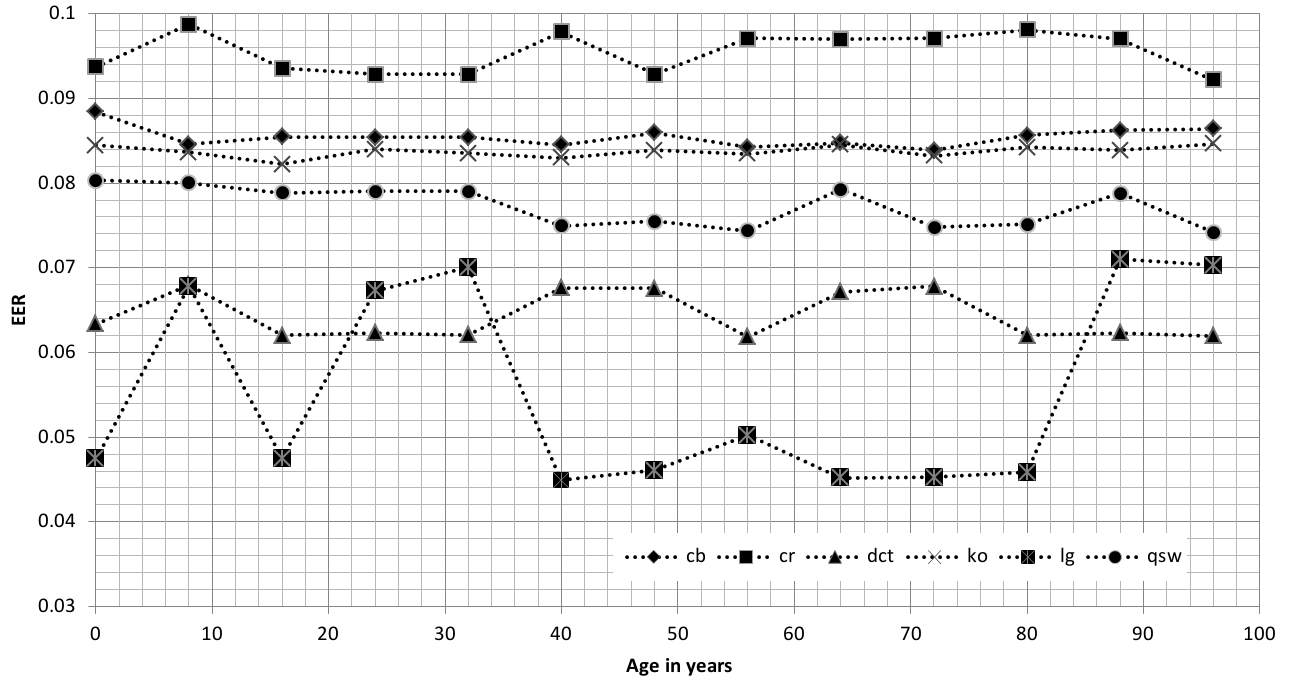
\includegraphics[width=\linewidth]{img/sensor1.png}
  \caption{EER using Sensor A and WAHET segmentation }
  \label{fig:sensor1}
\end{figure}
 
 
 \subsection{Limitation of the results}
 \begin{itemize}
  \item Only one sensor tested (probably not representative)
  \item In-Camera fixing of sensor defects neglected (might influence development rate, but not so important, because also tested with multiples of the original rate)
  \item Always same settings in camera?!
  \item unsure whether noise reduction on in iris sensors
  \item But proved in JLEUNG that was off... so these rates probably representative
  \item segmentation or iris code?
 \end{itemize}
 
 
 \section{Conclusion}
 \label{conclusion}
 We used a simulation to embed aging-related defects onto a sensors output. Practical relevance of the simulation has been established by retrieving simulation parameters from data, which has been captured by an iris scanner in a 4 years' difference. To retrieve these parameters, a method was proposed in section \ref{hotPixelRate}. By using these parameters and similar ones from related work, an experiment has been carried out. In this experiment the impact of sensor-aging on the accuracy of iris recognition systems was investigated.
 
 Interpreting the results, we can say that the LogGabor-1D method is vulnerable to aging-related defects. The algorithm's of Ma et al, Monro at al and Rathgeb and Uhl's DCT based algorithm are rather stable, whereas Rathgeb and Uhl's context based algorithm and the algorithm of Ko at al is considered to be robust. However, no tendency to a overall decrease in recognition accuracy can be determined. 
 In conclusion, this paper shows that some algorithms are more vulnerable to age-related defects than others, although no general tendency in accuracy can be observed. 
 

 %\section{Future work}
 %\begin{itemize}
 % \item Detect hot/stuck pixels by laboratory measurements. Compare to the observed method
 % \item Also no true stuck pixel http://euler.ecs.umass.edu/research/ctkk-spie-2013.pdf
 %\end{itemize}


% ------------------------ Reference section

{\small
\bibliographystyle{ieee}
\bibliography{egbib}
}

% TODO: Table referencing does not work!!
% TODO: Figure 2 enhance

\end{document}
